% 2007 年广东卷文科第 17 题：几何体的俯视图（8×6 矩形及两条对角线）。
% 来源 PDF：gaokaomath-src/普通高考/2007/2007广东文.pdf
% SHA-256：6c8a7179f8b64b91f8f189f0aca7da3523d5d42dd5b8d2c8e9c0d3c6998459ee
% 原页：2007广东文.pdf 第 2 页（A3 三栏）第 1 栏，书页码 374。
% 重绘依据：矩形长 8、宽 6，两条对角线为原图所画；尺寸线标注在下方与右侧。
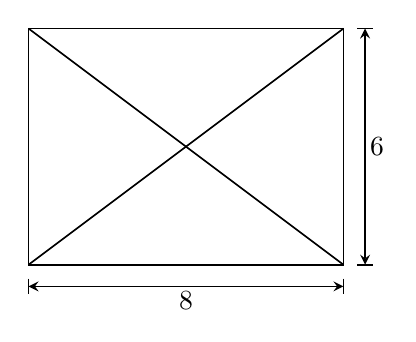
\begin{tikzpicture}[x=0.5cm, y=0.5cm, semithick,
  every node/.style={inner sep=1.5pt}]

  \draw (0,0) rectangle (8,6);
  \draw (0,0) -- (8,6);
  \draw (0,6) -- (8,0);

  % 下方尺寸线 8
  \draw[<->,>=stealth] (0,-0.55) -- (8,-0.55);
  \draw (0,-0.35) -- (0,-0.75);
  \draw (8,-0.35) -- (8,-0.75);
  \node[below] at (4,-0.55) {$8$};

  % 右侧尺寸线 6
  \draw[<->,>=stealth] (8.55,0) -- (8.55,6);
  \draw (8.35,0) -- (8.75,0);
  \draw (8.35,6) -- (8.75,6);
  \node[right] at (8.55,3) {$6$};
\end{tikzpicture}
